\section{\label{sec 4}Моделирование распада произвольного разрыва}

\subsubsection{Вход в двухфазную область жидкость-газ}

Было проведено МД-моделирование входа изоэнтропы разгрузки алюминия в двухфазную область жидкость–газ. Начальные характеристики исследуемого металла $Mo$ были следующими: $T_{sample, t=0} = 5$ и $\rho_{sample, t=0} = 1.25$; а соответствующие характеристики барьера из атомов $Ar$: $T_{barrier, t=0} = 0.7$ и $\rho_{barrier, t=0} = 0.001$.

\begin{figure*}[ht]
    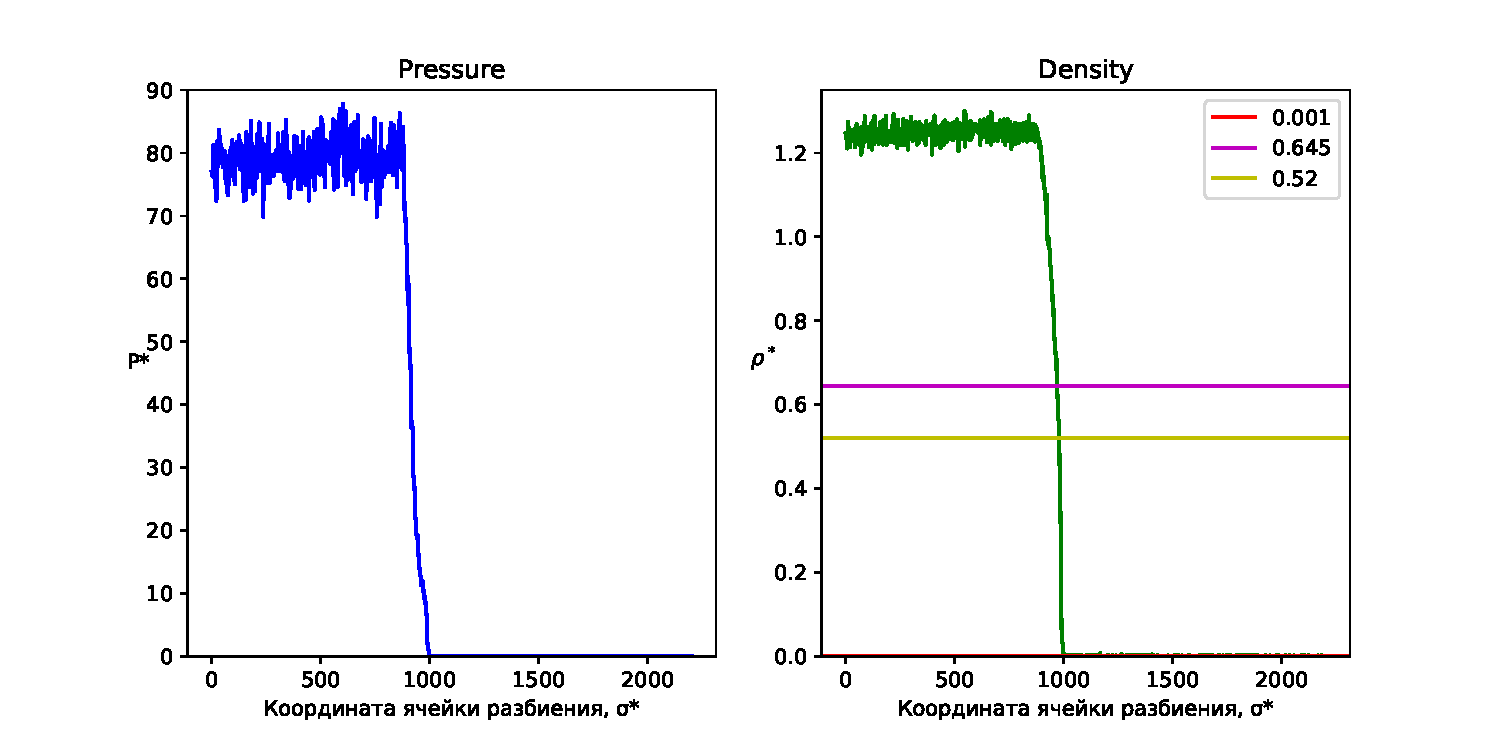
\includegraphics[width=\linewidth]{img/example_0.001/relax_wave3850.pdf}
    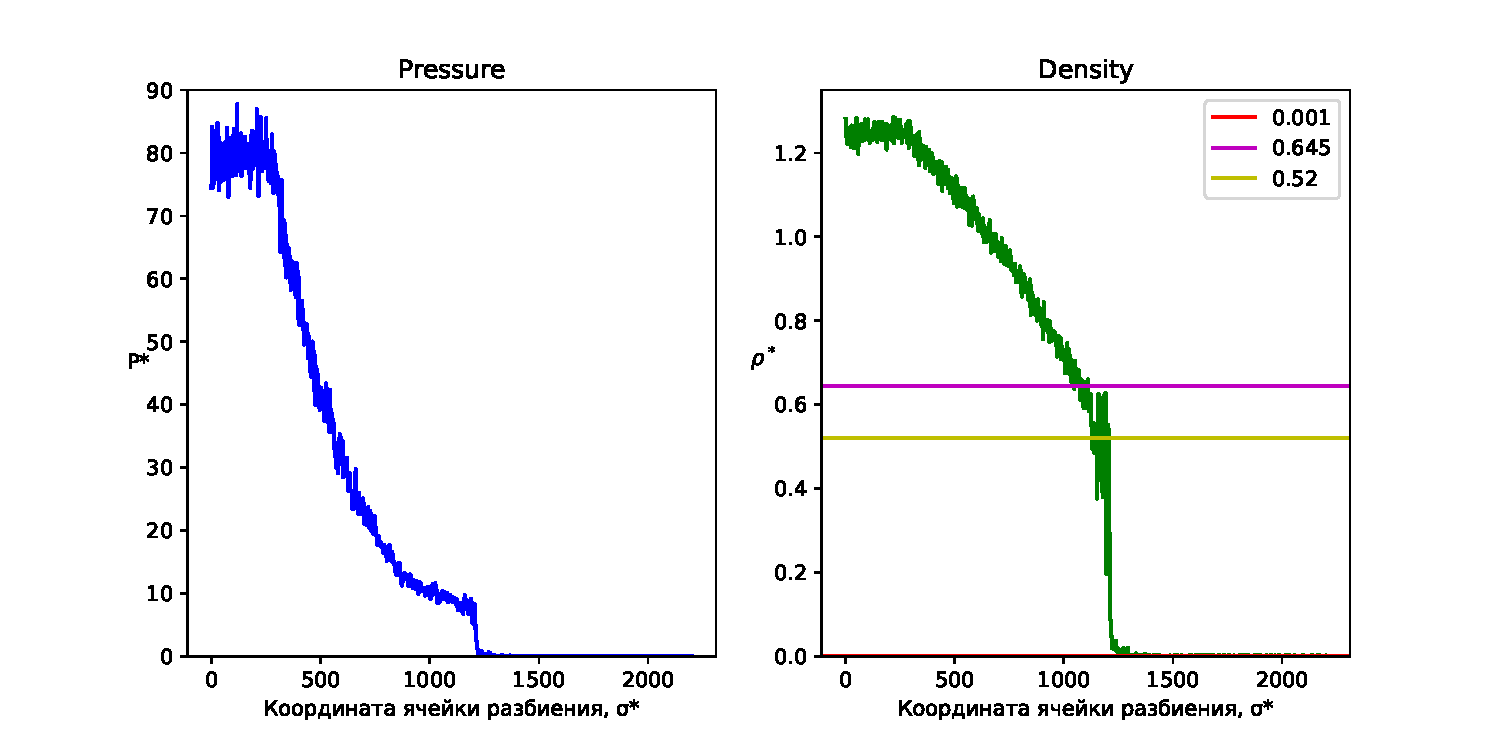
\includegraphics[width=\linewidth]{img/example_0.001/relax_wave36650.pdf}
    \caption{\label{fig:s_0.001} Моделирование в режиме ударной трубы, профили давления и плотности: верхний на шаге 3850, нижний на шаге 36650. Две горизонтальные линии на графике плотности обозначают, обсужденное ранее, значение плотности в точки пересечения изоэнтропы с бинодалью и значение плотности в образце, после прохождения по нему волны разрежения.}
\end{figure*}

Профили давления и плотности, полученные на разных этапах моделирования, представлены на рисунке \ref{fig:s_0.001}. Рассмотрим более детально полученные графики, в результате распада произвольного разрыва в области образца $Reg_{sample}$, состоящей из атомов $Mo$, и в области преграды $Reg_{barrier}$, состоящей из атомов $Ar$. В $Reg_{sample}$ наблюдаются плавные изменения распределения параметров $𝑃$ и $\rho$ относительно начальных значений, причем профили соответствуют движению волны разрежения влево от поверхности разрыва. В $Reg_{barrier}$, напротив, наблюдаются скачкообразные изменения этих параметров, что свидетельствует движению ударной волны сжатия вправо от поверхности разрыва. Значение плотности образца за волной разряжения, в приведённом эксперименте, соответственно равняется $0.52$. Полученная величина является меньшей по сравнению со значением плотности $0.645$ в точке пересечения изоэнтропы с бинодалью, что свидетельствует о проникновении внутрь двухфазной области жидкость-газ.

\begin{figure*}[ht]
    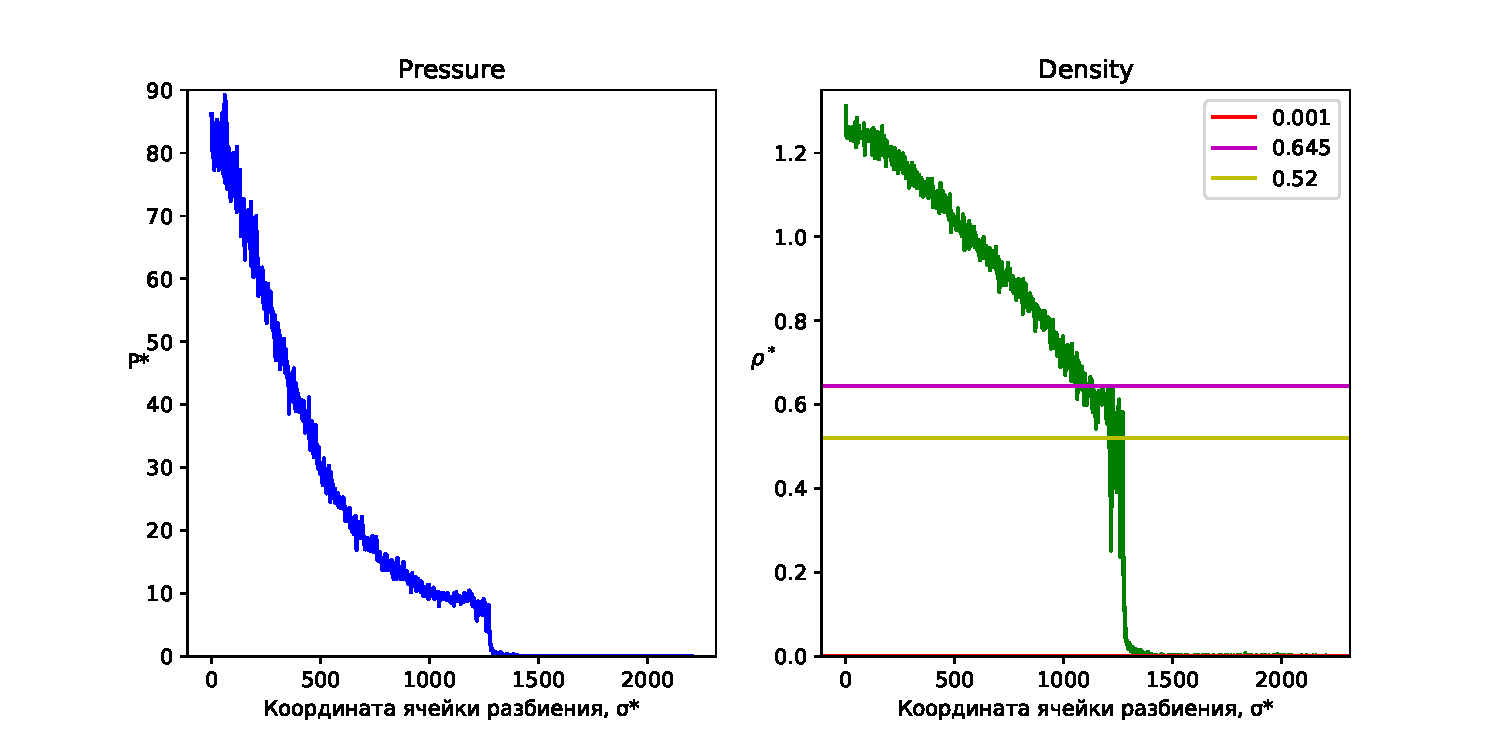
\includegraphics[width=\linewidth]{img/example_0.001/relax_wave46650.pdf}
    \caption{\label{fig:s_0.001_46650} Моделирование в режиме ударной трубы, профили давления и плотности на шаге 46650. Две горизонтальные линии на графике плотности обозначают, обсужденное ранее, значение плотности в точки пересечения изоэнтропы с бинодалью и значение плотности в образце, после прохождения по нему волны разрежения.}
\end{figure*}

Однако дальнейшее моделирование (рис. \ref{fig:s_0.001_46650}) показывает, что однородное состояние не успевает сформироваться. На графике плотности наблюдаются сильные флуктуации внутри двухфазной области. Однородное состояние быстро разрушается, и система стремится вернуться в более стабильную однофазную область. 

\subsubsection{Исследование волнового течения на границе двухфазной области}

С целью выяснения причины расхождения теоретического гидродинамического решения задачи распада произвольного разрыва и непосредственных результатов проведённого эксперимента была проведена серия моделирований с использованием преград различной плотности, чтобы проанализировать эффекты возникающие внутри двухфазной области, препятствующие образованию однородного состояния. 

\begin{figure}[ht]
    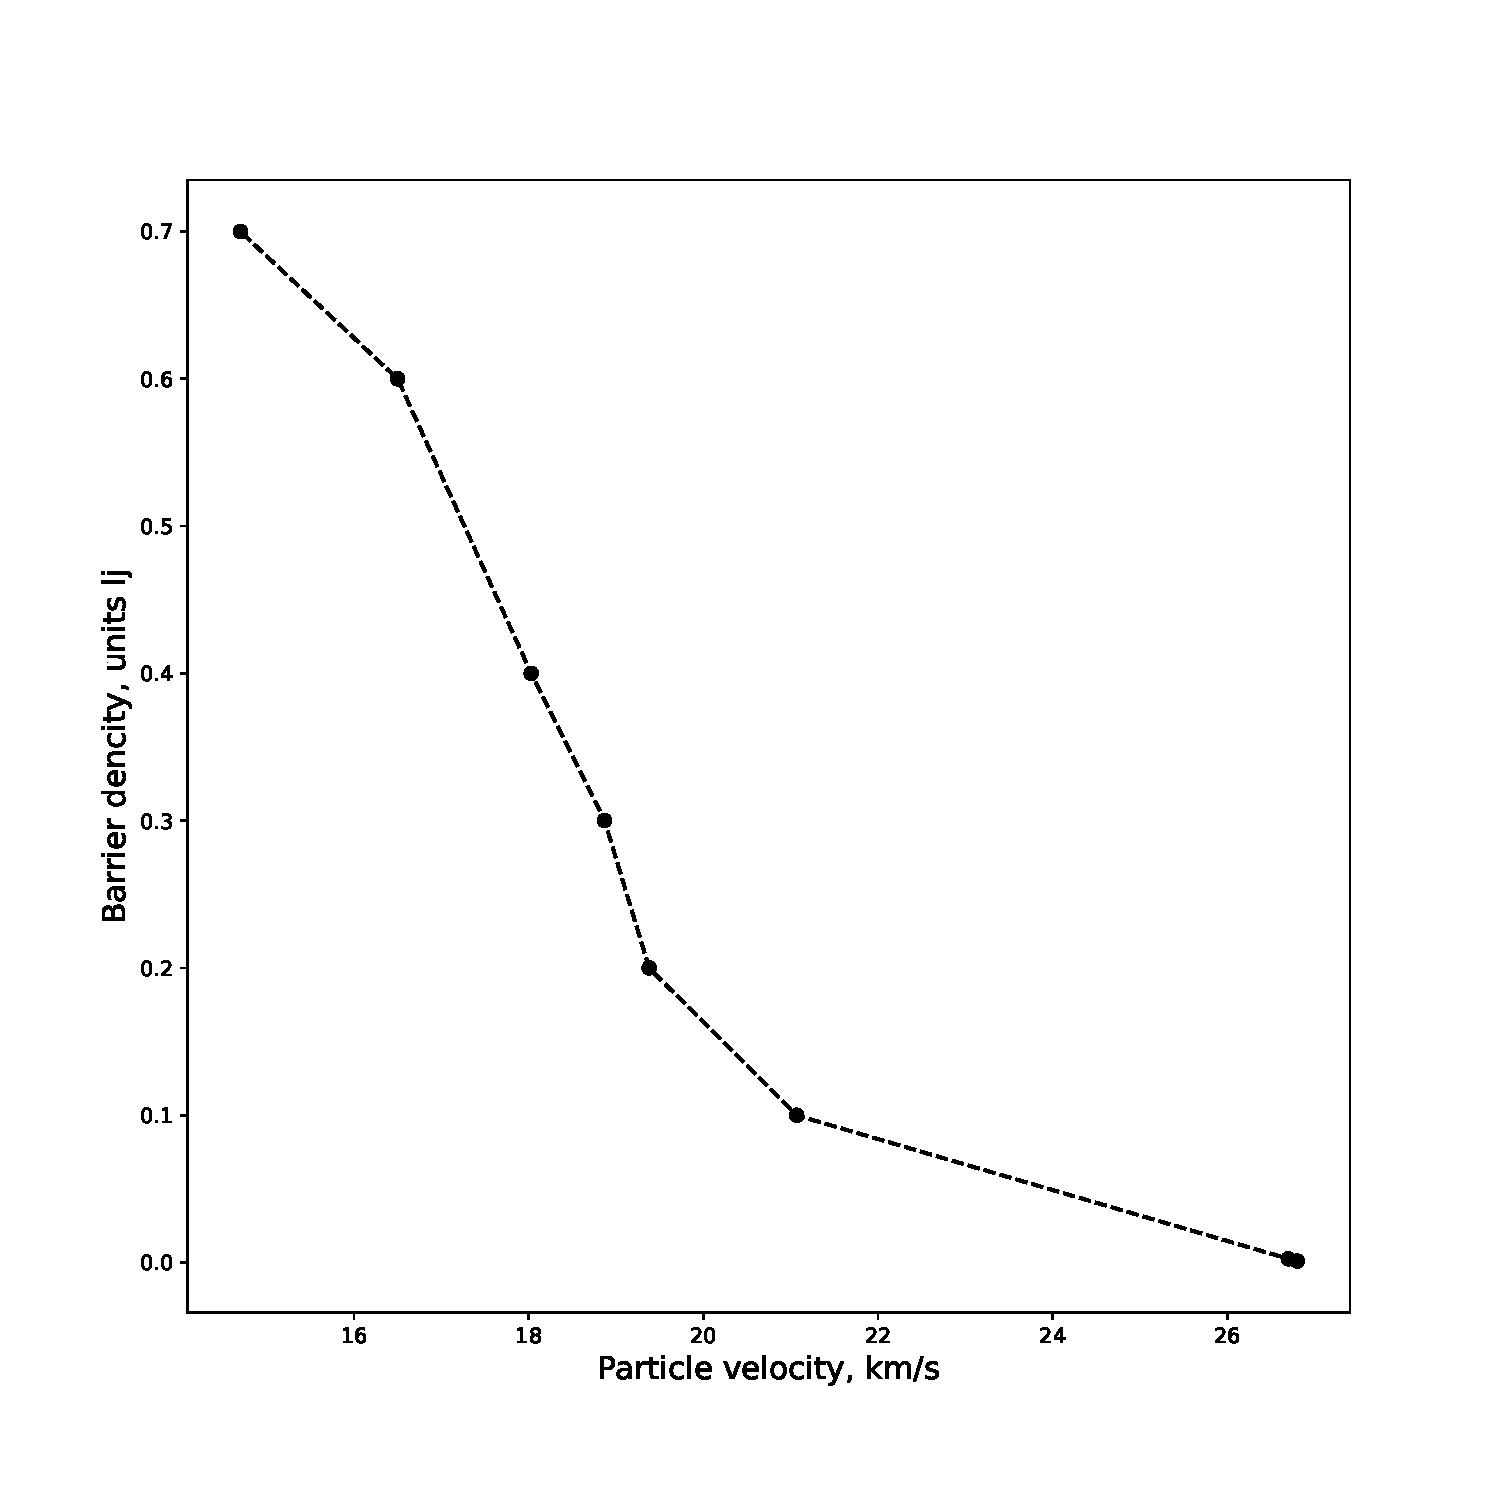
\includegraphics[width=\linewidth]{img/speed_comp.pdf}
    \caption{\label{fig:speed} График зависимости скорости распространения ударной волны в преграде.}
\end{figure}

На приведённом рисунке \ref{fig:speed} заметен характерный излом на изоэнтропе разгрузки, при использовании преград малой плотности. Как было показано ранее, данные значения плотности, позволяют веществу после разгрузки попасть внутрь двухфазной области. Однако изменение скорости распространения вещества перед фронтом ударной волны, указывает на образование быстрый излёт частиц вглубь невозмущённого вещества, приводящий к образованию струевидных течений. 